\section{Triangle expansions and sharp face codimension}
\label{ex:sec-triangle-expansions}

Extremal rank examples already occur among the cubic staircases of
Abdi et al.~\cite[discussion after Corollary~6.6 and Figure~2]{AbdiCornuejolsDadushDalirrooyfard2026}.
They have exactly three perfect matchings meeting every minimum odd
cut once, and those cut rows have rank \(|E|-2\).
We give an explicit triangle-expansion construction and derive the
associated prescribed-marginal entropy formulas. This also gives
a necessary lower bound on a universal entropy coefficient.
The construction underlying Klee graphs is standard;
see Cygan, Pilipczuk, and \v{S}krekovski
\citep[Section~1 and Lemma~2.1]{CyganPilipczukSkrekovski2013}
on the triangle expansions and the unique partition into three perfect
matchings, up to permutation. We give the construction and the argument
needed here. Balanced matching laws on cubic graphs and triangle
contractions also occur in the corrected full version of
Esperet et al.~\cite[Claim~3 and Lemma~10]{EsperetEtAl2011}.
Although an expansion can introduce further perfect
matchings, the prescribed uniform edge marginals force a law to
remain on three of them.

We retain \(P(G)\), \(a(M)\), \(F_x\), and \(d(x)=\dim F_x\)
from Section~\ref{geom:sec-polytope}, and the entropy functions
\(F,B,H\) from Equations~\eqref{intro:H}--\eqref{intro:FB}.
The separable comparison considered below is
\(H(x)\ge F(x)-cB(x)\). All edge labels, including parallel-edge
labels, are retained.

\subsection{Expansion and contraction}

Let \(v\) be a vertex of degree three in a loopless multigraph
\(G\) that has a perfect matching, with incident labelled edges
\(e_i=vu_i\), \(1\le i\le3\).
The vertices \(u_i\) need not be distinct. Replace \(v\) by a
triangle on new vertices \(t_1,t_2,t_3\), reattach \(e_i\) to
\(t_i u_i\), and let \(f_i\) denote the triangle edge opposite
\(t_i\). Call the resulting graph \(G'\), and set
\(T=\{t_1,t_2,t_3\}\). Reattached edges keep their old labels;
the \(f_i\) receive new labels. Figure~\ref{ex:fig-triangle-expansion}
shows the local change.

Every perfect matching \(M\) of \(G\) contains exactly one of
\(e_1,e_2,e_3\), say \(e_i\). Its unique extension that crosses
\(\delta(T)\) once is obtained by retaining its labelled edges
and adding \(f_i\). Conversely, contracting \(T\) in a perfect
matching of \(G'\) that crosses \(\delta(T)\) once recovers
exactly one perfect matching of \(G\).

\begin{figure}[htbp]
\centering
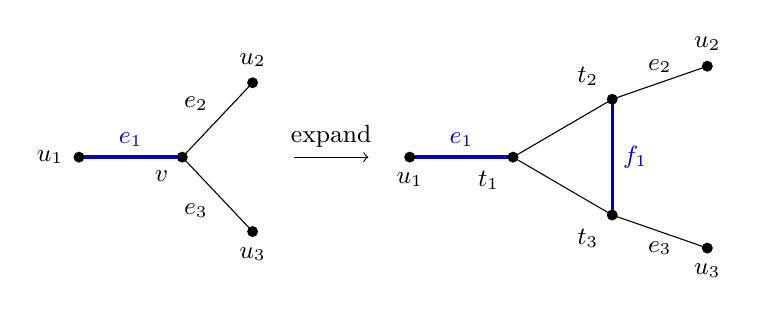
\begin{tikzpicture}[
  x=1.05cm,y=1.05cm,
  matched/.style={very thick,blue!75!black},
  vertex/.style={circle,fill,inner sep=1.4pt},
  every node/.style={font=\small}
]
  \coordinate (v) at (0,0);
  \coordinate (u1) at (-1.25,0);
  \coordinate (u2) at (0.85,0.9);
  \coordinate (u3) at (0.85,-0.9);
  \draw[matched] (u1)--node[above] {\(e_1\)} (v);
  \draw (u2)--node[above left] {\(e_2\)} (v);
  \draw (u3)--node[below left] {\(e_3\)} (v);
  \node[vertex,label=below left:\(v\)] at (v) {};
  \node[vertex,label=left:\(u_1\)] at (u1) {};
  \node[vertex,label=above:\(u_2\)] at (u2) {};
  \node[vertex,label=below:\(u_3\)] at (u3) {};

  \draw[->] (1.35,0)--node[above] {expand} (2.25,0);

  \coordinate (t1) at (4,0);
  \coordinate (t2) at (5.2,0.7);
  \coordinate (t3) at (5.2,-0.7);
  \coordinate (w1) at (2.75,0);
  \coordinate (w2) at (6.35,1.1);
  \coordinate (w3) at (6.35,-1.1);
  \draw[matched] (w1)--node[above] {\(e_1\)} (t1);
  \draw (w2)--node[above] {\(e_2\)} (t2);
  \draw (w3)--node[below] {\(e_3\)} (t3);
  \draw (t1)--(t2) (t1)--(t3);
  \draw[matched] (t2)--node[right] {\(f_1\)} (t3);
  \node[vertex,label=below left:\(t_1\)] at (t1) {};
  \node[vertex,label=above left:\(t_2\)] at (t2) {};
  \node[vertex,label=below left:\(t_3\)] at (t3) {};
  \node[vertex,label=below:\(u_1\)] at (w1) {};
  \node[vertex,label=above:\(u_2\)] at (w2) {};
  \node[vertex,label=below:\(u_3\)] at (w3) {};
\end{tikzpicture}
\caption{A local triangle expansion. The displayed matching uses
\(e_1\); its unique extension crossing the triangle cut once
adds the opposite edge \(f_1\). Thick blue edges are selected.
The rest of the graph is unchanged.}
\label{ex:fig-triangle-expansion}
\end{figure}


\begin{samepage}
\begin{lemma}[The face of a triangle expansion]
\label{ex:lem-expansion-face}
The set
\[
 Q_T=\{y\in P(G'):y(\delta(T))=1\}
\]
is a face of \(P(G')\) affinely isomorphic to \(P(G)\). Under this
isomorphism an old edge keeps its coordinate and
\[
 y_{f_i}=y_{e_i}\qquad(1\le i\le3).
\]
If \(x\in P(G)\) has coordinate \(1/3\) on every edge, its image
\(x'\) has coordinate \(1/3\) on every edge of \(G'\).
The isomorphism maps the minimal face at \(x\) onto the minimal
face at \(x'\).
\end{lemma}
\end{samepage}

\begin{proof}
Every perfect matching of \(G'\) crosses the odd cut
\(\delta(T)\) either once or three times. Hence
\(y(\delta(T))\ge1\) is valid on \(P(G')\), and its equality set
is a face. A convex combination lies in this face exactly when
every matching with positive coefficient crosses the cut once.
For these matchings the extension and contraction just described
are inverse bijections, and the indicator of \(f_i\) equals the
indicator of \(e_i\). They therefore induce the stated affine
isomorphism, with inverse given by restriction to the old edge
labels.

The coordinate statement follows directly. Finally, \(Q_T\) is
a face containing \(x'\). The minimal face of \(P(G')\) at
\(x'\) is therefore also the minimal face of \(Q_T\) at \(x'\);
affine isomorphisms preserve minimal faces.
\end{proof}

\subsection{A triangular minimal face for every order}

Begin with two vertices joined by three distinct labelled parallel
edges. Its three one-edge perfect matchings partition its edge set.
Repeatedly expand any vertex as above. Each expansion adds two
vertices and three edges, and all degrees remain three. Denote
any graph obtained after \(m-1\) expansions by \(G_m\), so that
\[
 |V(G_m)|=2m,\qquad |E(G_m)|=3m.
\]
The three initial perfect matchings extend uniquely at each step.
Their extensions \(M_1,M_2,M_3\) still partition the edge set:
the old edges retain their partition, and \(f_i\) belongs to the
extension of the matching containing \(e_i\). In particular,
\[
 x^{(m)}=\tfrac13\bigl(a(M_1)+a(M_2)+a(M_3)\bigr)
\]
has every coordinate equal to \(1/3\) and belongs to the full
perfect-matching polytope.

The first expansion gives \(K_4\); subsequent expansions preserve
simplicity. Thus \(G_m\) is simple for every \(m\ge2\), and these
are Klee graphs. Only the starting case \(m=1\) needs parallel
edges.

\begin{proposition}[Sharp codimension and prescribed-marginal entropy]
\label{ex:prop-klee-face}
For every integer \(m\ge1\), the graph \(G_m\) and the point
\(x^{(m)}\) above satisfy
\[
 F_{x^{(m)}}=
 \operatorname{conv}\{a(M_1),a(M_2),a(M_3)\},
 \qquad d(x^{(m)})=2.
\]
The unique law on perfect matchings with mean \(x^{(m)}\) is the
uniform law on \(M_1,M_2,M_3\). Consequently,
\begin{equation}
\label{ex:eq-klee-values}
 \begin{aligned}
 |E(G_m)|-d(x^{(m)})&=3m-2,\\
 H(x^{(m)})&=\ln3,\\
 F(x^{(m)})&=m\ln3,\\
 B(x^{(m)})&=2m\ln(3/2).
 \end{aligned}
\end{equation}
\end{proposition}

\begin{proof}
For \(m=1\), the three matching vectors are the three coordinate
vectors in \(\mathbb R^3\), and \(P(G_1)\) is their simplex.
Its uniform point is in its relative interior. Repeated application
of Lemma~\ref{ex:lem-expansion-face} shows that the minimal face at
\(x^{(m)}\) is the image of this simplex, with vertices
\(a(M_1),a(M_2),a(M_3)\). In particular its dimension is two.

One can also see the restriction on laws directly. For the last
inserted triangle, a law with edge marginals \(1/3\) has expected
cut-crossing count \(3(1/3)=1\). Since each matching crosses this
cut once or three times, it must cross once almost surely.
Contraction gives a law on the preceding graph with the same
uniform marginals, and the crossing-one extension is unique.
Iterating leaves only the three initial matchings. Thus the
original law is supported on \(M_1,M_2,M_3\). Since these
matchings partition the edges, the marginal of any edge in
\(M_i\) equals the probability assigned to \(M_i\), which must
be \(1/3\). This proves uniqueness and the entropy formula.

There are \(3m\) edges, all with marginal \(1/3\). Substitution
in the definitions of \(F\) and \(B\) gives the remaining
formulas.
\end{proof}

All coordinates here are strictly between zero and one.
Equation~\eqref{ex:eq-klee-values} therefore attains the bound in
Proposition~\ref{geom:prop-rank} for every \(m\ge1\). Equivalently,
by Equation~\eqref{geom:eq-rank}, the tight odd-cut rows have rank
\(3m-2\). The dimension two is the dimension of the minimal face
at \(x^{(m)}\); the whole perfect-matching polytope can have
additional vertices.

\begin{corollary}[Restriction on a universal entropy coefficient]
\label{ex:cor-coefficient}
If a constant \(c\) satisfies
\[
 H(x)\ge F(x)-cB(x)
\]
for every finite loopless multigraph \(G\) and every
\(x\in P(G)\), then
\[
 c\ge\frac{\ln3}{2\ln(3/2)}.
\]
The same necessary bound holds if the assertion is restricted to
simple graphs.
\end{corollary}

\begin{proof}
Applying the asserted inequality to \(G_m,x^{(m)}\) gives
\[
 c\ge
 \frac{(m-1)\ln3}{2m\ln(3/2)}.
\]
Let \(m\) tend to infinity. The graphs with \(m\ge2\) are simple,
so the same limit applies under that restriction.
\end{proof}

The necessary coefficient in Corollary~\ref{ex:cor-coefficient} lies
strictly between $1$ and the universal coefficient $2$ supplied by
Theorem~\ref{ent:main}. Sharpness of the geometric estimate therefore
does not settle the optimal entropy coefficient. The next example makes
the failure of coefficient one explicit at a fixed order.

\subsection{An eight-vertex obstruction to coefficient one}

For a concrete instance, take vertex set \(\{0,1,\ldots,7\}\) and
edge set
\[
 E=\{01,03,05,14,16,23,24,27,34,56,57,67\},
\]
where \(ij\) denotes the undirected edge with endpoints \(i,j\).
Contracting the triangles \(T=\{2,3,4\}\) and
\(U=\{5,6,7\}\) gives \(K_4\). Thus this graph is obtained by
expanding two vertices of \(K_4\), and is an instance of \(G_4\).

Its five perfect matchings are
\[
 \begin{aligned}
 M_1&=\{01,27,34,56\},&
 M_2&=\{03,16,24,57\},\\
 M_3&=\{05,14,23,67\},&
 N_1&=\{03,14,27,56\},\\
 &&N_2&=\{05,16,27,34\}.
 \end{aligned}
\]
This list follows without enumeration software. A matching uses
one of \(01,03,05\). If it uses \(01\), the remaining two odd
triangles are joined only by \(27\), forcing \(M_1\). If it uses
\(03\), vertex \(1\) is matched by \(14\) or \(16\), after which
the remaining edges are forced, giving \(N_1\) or \(M_2\).
If it uses \(05\), the same two choices at vertex \(1\) force
\(M_3\) or \(N_2\).

The cuts
\[
 \delta(T)=\{03,14,27\},\qquad
 \delta(U)=\{05,16,27\}
\]
both have total marginal one at \(x_e=1/3\).
The matching \(N_1\) crosses the first cut three times, and
\(N_2\) crosses the second cut three times. They therefore have
probability zero in every law with those marginals. The remaining
three matchings partition \(E\), so their probabilities are all
\(1/3\). In particular the relevant entropy is \(\ln3\), even
though the graph has five perfect matchings in total.

At this feasible point of the full polytope,
\[
 H(x)=\ln3,\qquad
 F(x)-B(x)=4\ln(4/3)>\ln3,
\]
because \( (4/3)^4=256/81>3\).
The difference \(F(x)-B(x)-H(x)\) is
\(\ln(256/243)>0\). This gives a simple eight-vertex
counterexample to the coefficient-one lower bound.
